\documentclass[12pt,a4paper]{article}

% Page layout
\usepackage[margin=1in]{geometry}
\usepackage{setspace}
\onehalfspacing

% Tables and figures
\usepackage{graphicx}
\usepackage{booktabs}
\usepackage{float}
\usepackage{longtable}
\usepackage{array}

% Maths and citations
\usepackage{amsmath}
\usepackage{natbib}
\usepackage{hyperref}

% Title
\title{Socioeconomic Predictors of Electoral Competitiveness in Bangladesh: 
A Constituency-Level Study for the 2026 Election Context}

\author{Md Ashraful Alam Gazi}
\date{\today}

\begin{document}

\maketitle

\begin{abstract}

This study examines whether constituency-level socioeconomic and security conditions are associated with electoral competitiveness in Bangladesh in the 2026 election context. Using a newly constructed dataset of 297 parliamentary constituencies, the paper combines election outcome variables with demographic and household indicators from the Bangladesh Population and Housing Census 2022, constituency-level crime rates, metro status, and a district-level remittance proxy. Electoral competitiveness is measured through winner vote share and victory margin. The analysis estimates three Ordinary Least Squares models using HC3 robust standard errors, followed by diagnostic tests, robustness checks, and supplementary binary logistic regression models.

The results show that population density and total crime rate are the most consistent predictors of electoral competitiveness. In the main margin model, population density is negatively associated with victory margin, with a coefficient of approximately -0.0003, meaning that an increase of 1,000 people per square kilometre is associated with about a 0.3 percentage-point reduction in the victory margin. Total crime per 100,000 people is also negative and statistically significant, with a coefficient of approximately -0.3285. Model 3 explains around 10.5 percent of the variation in constituency-level victory margins. By contrast, household size, literacy rate, violent crime rate, metro status, and remittance do not show robust statistically significant relationships in the main OLS models. Robustness checks confirm that total crime is the most stable predictor, while the population-density result is somewhat sensitive to functional form. A supplementary binary logit model also shows that denser constituencies are more likely to fall within the closest-margin category.

Overall, the findings suggest that electoral competitiveness in Bangladesh is more strongly associated with local demographic concentration and broader recorded crime conditions than with remittance exposure. The study does not claim causality, and the district-level measurement of remittance limits constituency-level interpretation. Nevertheless, the paper provides a constituency-level empirical framework for studying how local structural conditions are linked to electoral competition in Bangladesh.

\end{abstract}

\section{Introduction}

\subsection{Background}

Elections are often explained through national-level political factors such as party competition, leadership, alliances, campaign strategy, and voter turnout. These factors are important, but they do not fully explain why electoral competition varies across constituencies. Some constituencies are won by narrow margins, while others are won comfortably. Bangladesh's electoral politics has also been shaped by party organisation, political polarisation, and changing democratic institutions \citep{jahan2014,riaz2019}. Therefore, constituency-level analysis should be understood as a complement to, rather than a replacement for, national political explanations. This variation suggests that local constituency-level conditions may also matter.

This paper examines electoral competitiveness in Bangladesh using a constituency-level dataset prepared for the 2026 election context. The study links electoral outcomes with demographic, socioeconomic, crime, metro, and remittance-related indicators. The demographic and household variables are mainly drawn from the Bangladesh Bureau of Statistics (BBS) \textit{Population and Housing Census 2022}, which provides official information on population, household characteristics, literacy, employment, urban-rural location, and foreign-remittance-recipient households \citep{bbs2023}. The final analysis sample includes 297 valid constituencies after excluding Chittagong-2, Chittagong-4, and Sherpur-3 because of incomplete or unsuitable data for the final regression sample.

The theoretical starting point of this paper comes from rational-choice approaches to electoral behaviour. Downs argues that political parties and voters operate under uncertainty, and that political behaviour depends on information, perceived benefits, and the available alternatives \citep{downs1957}. This matters for constituency-level analysis because local conditions may shape both voter behaviour and party strategy. In dense, urbanised, or politically contested constituencies, parties may campaign differently and voters may be exposed to different levels of information, mobilisation, and competition.

At the same time, elections should not be treated only as mathematical outcomes. The review of Banerjee's \textit{Why India Votes} highlights that elections are also social, cultural, and moral events, where voters attach meaning to participation, recognition, protest, loyalty, citizenship, and duty \citep{das2015}. This is important for the present study because regression models can identify statistical patterns, but they cannot fully capture the lived political experience of voters. Therefore, this paper uses quantitative methods while recognising that electoral behaviour is shaped by broader social and political contexts.

\subsection{Research Problem}

Most public discussion of Bangladeshi elections focuses on parties, candidates, alliances, and national political developments. These explanations are necessary but incomplete. They do not fully address why some constituencies are consistently more competitive than others. Electoral competitiveness is commonly studied through the closeness of contest between candidates or parties, especially at the district or constituency level \citep{blais2009,cox2020}. This makes victory margin an appropriate measure for examining why some constituencies are more closely contested than others. A constituency-level approach can add value by examining whether measurable local characteristics are associated with winner vote share and victory margin.

The research problem is therefore empirical: are socioeconomic, demographic, and local contextual variables associated with electoral competitiveness in Bangladesh? This paper examines whether population density, household size, literacy rate, crime rates, metro status, and remittance exposure are related to winner vote share and victory margin.

The inclusion of crime-related variables is motivated by wider South Asian electoral literature. Vaishnav's work on India shows that crime, money, local power, candidate reputation, and party strategy can interact within an electoral marketplace \citep{vaishnav2017}. His argument does not imply that the same mechanisms operate identically in Bangladesh, but it provides a useful regional framework for treating crime as a politically relevant constituency-level condition. In this paper, crime is not treated as a direct cause of election results. Rather, it is tested as a contextual variable that may be associated with narrower or wider victory margins.

The inclusion of remittance is motivated by the economic voting literature and by the importance of migration income in Bangladesh. Oganesyan argues that economic voting research has focused heavily on developed democracies, while developing-country contexts may differ because voters face greater economic volatility, weaker party institutionalisation, and different patterns of retrospective and prospective evaluation \citep{oganesyan2014}. Since remittance can influence household welfare and local economic conditions, it is included as an exploratory predictor. However, because the remittance variable used in this study is measured at the district level, it is interpreted as a proxy rather than a direct constituency-level income measure.

\subsection{Research Question and Objectives}

The main research question of this paper is:

\begin{quote}
Which constituency-level socioeconomic and demographic factors are associated with electoral competitiveness in Bangladesh?
\end{quote}

The study has five objectives. First, it builds a constituency-level dataset that combines election outcomes with demographic, crime, metro, and remittance indicators. Second, it examines the distribution of key variables through descriptive statistics, correlation analysis, party-wise comparisons, metro versus non-metro comparisons, and scatterplots. Third, it estimates OLS regression models for winner vote share and victory margin. Fourth, it evaluates the reliability of the main findings through diagnostic tests and robustness checks. Fifth, it uses binary logistic regression models as supplementary evidence to identify whether the same predictors help classify highly competitive constituencies.

\subsection{Contribution of the Study}

This paper contributes to the study of electoral politics in Bangladesh in three ways. First, it shifts attention from national-level political narratives to constituency-level empirical analysis. Second, it links election results with official demographic and household indicators from BBS Census 2022, along with crime and remittance variables. Third, it combines exploratory data analysis, OLS regression, diagnostic testing, robustness checks, and binary competitiveness models.

The central finding is that population density and total crime rate are the most consistent predictors of electoral competitiveness in the dataset. Higher population density and higher total crime rates are generally associated with narrower victory margins. Remittance exposure does not show a robust statistically significant relationship in the main OLS models. These findings should be interpreted as statistical associations, not causal effects.

The remainder of the paper is structured as follows. Section 2 reviews the literature and develops the theoretical framework. Section 3 describes the data and variables. Section 4 explains the methodology. Section 5 presents the exploratory data analysis. Section 6 reports the regression results, diagnostics, robustness checks, and binary competitiveness models. Section 7 discusses the findings. Section 8 presents the limitations of the study. Section 9 concludes the paper and suggests directions for future research.

\section{Literature Review and Theoretical Framework}

\subsection{Electoral Competitiveness}

Electoral competitiveness refers to the degree to which an election is closely contested. The measurement of electoral competitiveness has received specific attention in comparative electoral research. District-level competitiveness can be measured through the closeness of electoral outcomes, including the gap between the winner and the nearest competitor \citep{blais2009,cox2020}. In this paper, victory margin is therefore used as the main indicator of constituency-level competitiveness. 

At the constituency level, the most direct measure of competitiveness is the victory margin between the winning candidate and the nearest competitor. A small margin indicates a competitive seat, while a large margin indicates a safer or less competitive seat. This paper therefore uses \textit{Margin\_Percentage} as the main dependent variable for electoral competitiveness.

Winner vote share is also useful because it shows the strength of the winning candidate. However, winner vote share and victory margin are closely related. A candidate who wins with a high vote share is usually more likely to win by a larger margin. For this reason, the two variables are not included together in the same regression model. Winner vote share is used in Models 1 and 2, while victory margin is used in Model 3 as the main competitiveness outcome.

The study of competitiveness matters because competitive constituencies are where political control is more uncertain. In such constituencies, parties and candidates may have stronger incentives to campaign, mobilise voters, and respond to local demands. In safer constituencies, the leading party or candidate may face weaker electoral pressure. Therefore, studying the predictors of competitiveness can help explain how local constituency conditions relate to the structure of electoral competition.

\subsection{Rational Voting, Uncertainty, and Information}

Downs provides an important theoretical foundation for this paper. His model treats parties and voters as actors operating under conditions of uncertainty \citep{downs1957}. Voters do not always possess complete information about government action, opposition alternatives, or the consequences of policies. Parties also face uncertainty about voter preferences, economic conditions, and the actions of their opponents. This makes information and political context central to electoral behaviour.

This framework is relevant for constituency-level analysis in Bangladesh. Constituencies differ in density, urbanisation, literacy, household structure, crime exposure, and remittance patterns. These factors may affect the local information environment and the way political competition operates. For example, densely populated constituencies may provide more opportunities for campaign contact, political discussion, media exposure, and voter mobilisation. Less dense constituencies may have different forms of local political organisation and social influence.

However, Downsian rational-choice theory should not be treated as a complete explanation of voting behaviour. It helps explain why information, uncertainty, and incentives matter, but it does not fully capture identity, emotion, loyalty, patronage, local reputation, or social pressure. This is why the present study uses rational-choice theory as a starting point, not as a complete theory of Bangladeshi voting behaviour.

\subsection{Elections as Social and Local Events}

The literature on South Asian elections also shows that elections are not only formal procedures or statistical outcomes. A review of Banerjee's \textit{Why India Votes} notes that elections can be understood as cultural and moral events, not only as exercises in representation and vote counting \citep{das2015}. The review highlights that voters may participate for several reasons, including instrumentality, loyalty, protest, recognition, peer pressure, citizenship, duty, and rights \citep{das2015}.

This perspective is important for the present paper because it places quantitative analysis in context. Regression models can identify whether variables such as population density, crime, and remittance are associated with competitiveness. They cannot fully explain why individual voters choose one candidate or party over another. The paper therefore avoids claiming that constituency-level variables directly determine voter behaviour. Instead, it treats them as structural and contextual indicators that may be associated with patterns of electoral competition.

\subsection{Economic Voting in Developing Democracies}

Economic voting theory argues that voters respond to economic conditions when making electoral choices. In many studies, elections are treated partly as judgements on economic performance. Oganesyan notes that most economic voting research has focused on developed democracies, while the developing world has received less attention \citep{oganesyan2014}. This matters because the assumptions developed in advanced democracies may not travel perfectly to developing-country contexts.

Developing democracies often face greater economic volatility, weaker institutionalisation, more fluid party systems, and different forms of voter-party linkage. Oganesyan argues that voters in developing countries may take the economy into account, but not always in the way predicted by classic economic voting theory \citep{oganesyan2014}. His findings suggest that voters in developing contexts may combine retrospective and prospective evaluations and may punish and reward incumbents asymmetrically.

The wider economic voting literature argues that voters may reward or punish governments based on economic performance, but the strength of this relationship depends on political and institutional context \citep{lewisbeck2000,duch2008}. In developing democracies, this relationship may be less straightforward because voters face different levels of economic volatility, party institutionalisation, and political accountability \citep{oganesyan2014}.

This supports the logic of including socioeconomic and economic-context variables in this study. Bangladesh is not analysed here through individual-level survey responses, so the paper cannot directly test whether voters personally reward or punish parties for economic conditions. Instead, it uses constituency-level indicators such as literacy, household size, density, and remittance exposure to examine whether local socioeconomic context is associated with electoral competitiveness.

\subsection{Population Density and Urbanisation}

Population density is one of the main predictors in this study. It captures how concentrated the population is within a constituency. Dense constituencies may differ from less dense constituencies in several politically relevant ways. They may contain more diverse occupational groups, stronger urban or semi-urban characteristics, more campaign activity, and more frequent social and political interaction.

Theoretically, higher density may increase competitiveness because parties can reach more voters in a smaller geographical space. Dense areas may also expose voters to more information, more political messaging, and more visible party competition. In this sense, population density is connected to the Downsian idea that information and uncertainty shape political behaviour \citep{downs1957}. When voters and parties operate in a more information-rich environment, electoral competition may become more intense.

District-level demographic structure can shape electoral contestation. Comparative research suggests that the size and demographic structure of electoral districts can influence the degree of political contestation \citep{gerring2015}. This supports the inclusion of population density as a core constituency-level predictor in this study.

However, density is not identical to metro status. Some dense constituencies may not be formally metropolitan, and some metro constituencies may include mixed socioeconomic populations. For this reason, the paper includes both \textit{Population\_Density} and a separate \textit{Metro} indicator.

\subsection{Crime and Political Competition}

Crime is included because the relationship between crime and politics is an important theme in South Asian electoral research. Vaishnav's work on India argues that criminality in politics should be understood through an electoral marketplace, involving both supply-side factors such as politicians and parties, and demand-side factors such as voters and local expectations \citep{vaishnav2017}. His argument is that criminal reputations may become politically useful in contexts where the rule of law is weak, social divisions are strong, or voters seek protection and local problem-solving. In Bangladesh, local political consolidation has also been shaped by informal power and patronage networks \citep{lewis2022}.

This does not mean that crime operates in the same way in Bangladesh. Nor does it mean that high-crime constituencies necessarily support criminal candidates. The relevance of Vaishnav's framework is broader: it shows that crime can be politically meaningful rather than merely a law-and-order statistic. Crime rates may reflect governance problems, contested local authority, social instability, or politically complex local environments.

This paper includes two crime variables: \textit{Total\_Crime\_per\_100k} and \textit{Violent\_Crime\_per\_100k}. Total crime captures the broader crime environment, while violent crime captures more severe forms of criminal activity. The expectation is that constituencies with higher crime rates may have narrower victory margins, either because they are more politically contested or because crime reflects deeper local instability. The analysis tests this as an association, not a causal claim.

\subsection{Remittance and Political Behaviour}

Remittance is included because migration income is economically important in Bangladesh and may affect household welfare, local development, and political expectations. Remittance may affect electoral behaviour indirectly by changing household welfare, economic security, and dependence on local political networks. However, because economic voting depends on institutional context and voter attribution of responsibility, the political effect of remittance is theoretically uncertain \citep{duch2008,lewisbeck2000,oganesyan2014}. BBS Census 2022 provides data on foreign-remittance-recipient general households by district and location in Table HH 14 \citep{bbs2023}. This allows the paper to include a remittance-related variable in the constituency-level dataset.

The variable used in this study is \textit{Log\_Remittance\_HH\_Total}, calculated using the log-transformed number of remittance-recipient households. The log transformation is used because raw remittance household counts are highly skewed. However, the variable is measured at the district level, not directly at the constituency level. This is a major limitation. It means that the variable should be interpreted as a district-level proxy for remittance exposure, not as a precise measure of constituency-level household income.

The expected relationship between remittance and electoral competitiveness is theoretically uncertain. Remittance may increase household economic security and reduce dissatisfaction, which could strengthen incumbent or dominant-party support. Alternatively, remittance may reduce dependence on local patronage, increase political independence, or raise expectations of accountability. Because of this ambiguity, and because the variable is district-level, this paper treats remittance as exploratory rather than as a core predictor.

\subsection{Theoretical Expectations and Hypotheses}

Based on the literature, the paper develops four hypotheses.

\textbf{H1: Population density and competitiveness.} Constituencies with higher population density are expected to have lower victory margins. This means that denser constituencies are expected to be more electorally competitive.

\textbf{H2: Crime and competitiveness.} Constituencies with higher total crime rates are expected to have lower victory margins. This means that higher-crime constituencies may be more electorally competitive.

\textbf{H3: Remittance and competitiveness.} Remittance exposure may be associated with electoral competitiveness, but the relationship is expected to be weaker and less stable because remittance is measured at the district level rather than the constituency level.

\textbf{H4: Metro status and competitiveness.} Metro constituencies may differ from non-metro constituencies in electoral competitiveness because metropolitan areas have different social, economic, and political characteristics.

These hypotheses are informed by three strands of literature: electoral competitiveness and district-level contestation \citep{blais2009,cox2020,gerring2015}, economic voting in developed and developing democracies \citep{lewisbeck2000,duch2008,oganesyan2014}, and South Asian work on patronage, local power, and crime-politics relationships \citep{kitschelt2007,vaishnav2017,lewis2022}. They are tested using descriptive analysis, OLS regression models, diagnostic tests, robustness checks, and supplementary binary logistic regression models. The aim is not to prove causal effects, but to identify whether systematic constituency-level relationships exist between socioeconomic conditions and electoral competitiveness.

\section{Data and Variables}

\subsection{Dataset Description}

This study uses a constituency-level dataset prepared for the Bangladesh 2026 election context. The unit of analysis is the parliamentary constituency. The main working file is \textit{Main\_Datasheet\_Rem.xlsx}, and the main analysis sheet is \textit{Analysis\_Data}. The final analysis sample includes 297 valid constituencies. Three constituencies, Chittagong-2, Chittagong-4, and Sherpur-3, were excluded because of incomplete or unsuitable data for the final regression sample.

The dataset combines electoral outcome variables with demographic, socioeconomic, crime, metro, and remittance-related indicators. The purpose of the dataset is not to predict the final outcome of the 2026 election, but to examine whether constituency-level conditions are statistically associated with electoral competitiveness.

\subsection{Data Sources}

The dataset was constructed from multiple sources. Election outcome variables were compiled at the constituency level. Demographic and household variables were taken from the Bangladesh Bureau of Statistics (BBS) \textit{Population and Housing Census 2022: National Report, Volume I} \citep{bbs2023}. This source provides official census indicators including population, household size, literacy, urban-rural location, and household-level characteristics. In particular, Table P35 provides household, population, household size, and literacy rate by upazila, while Table HH 14 provides foreign-remittance-recipient general households by district and location \citep{bbs2023}.

Crime variables were taken from the \textit{Crime Rate 2024} source used in the dataset construction \citep{crime2024}. The crime data were converted into rates per 100,000 population to make constituencies more comparable. This is important because raw crime counts are strongly affected by population size. A large constituency may naturally have more crimes in absolute terms, even if its crime risk is not higher. Using crime rates reduces this problem.

The remittance variable was added from BBS Census 2022 Table HH 14. However, this variable is available at the district level rather than directly at the constituency level. Therefore, remittance is used as a district-level proxy for remittance exposure. It should not be interpreted as a direct constituency-level income measure.

\subsection{Dependent Variables}

The study uses two main electoral outcome variables: \textit{Winner\_Vote\_Share} and \textit{Margin\_Percentage}.

\subsubsection{Winner Vote Share}

\textit{Winner\_Vote\_Share} measures the percentage of votes received by the winning candidate in each constituency. It captures the strength of the winner's electoral performance. A higher winner vote share indicates that the winning candidate secured a larger share of total votes.

This variable is used as the dependent variable in Model 1 and Model 2. It is useful because it shows whether constituency-level socioeconomic conditions are associated with the winning candidate's vote share.

\subsubsection{Victory Margin}

\textit{Margin\_Percentage} measures the percentage-point difference between the winning candidate and the nearest competitor. This is the main measure of electoral competitiveness in the paper. A lower margin means that the constituency is more competitive, while a higher margin means that the winner had a safer lead.

This variable is used as the dependent variable in Model 3. Since the central aim of the paper is to study electoral competitiveness, Model 3 is treated as the main regression model.

\subsubsection{Relationship Between Winner Vote Share and Victory Margin}

\textit{Winner\_Vote\_Share} and \textit{Margin\_Percentage} are closely related because both are derived from election results. A candidate with a very high vote share will often also have a large victory margin. For this reason, the two variables are not included together in the same regression model. Using both together would create a mechanical relationship and could distort the interpretation of the results.

\subsection{Independent Variables}

The independent variables are selected to capture constituency-level demographic, socioeconomic, crime, urbanisation, and remittance conditions. The main predictors are \textit{Population\_Density}, \textit{Household\_Size}, \textit{Literacy\_Rate}, \textit{Total\_Crime\_per\_100k}, \textit{Violent\_Crime\_per\_100k}, \textit{Metro}, and \textit{Log\_Remittance\_HH\_Total}.

\subsubsection{Population Density}

\textit{Population\_Density} measures the number of people per square kilometre. It is included because dense constituencies may have different political dynamics from less dense constituencies. Higher density may be associated with greater urbanisation, more campaign contact, more political communication, and more diverse voter groups. The theoretical expectation is that higher population density will be associated with lower victory margins, meaning greater electoral competitiveness.

\subsubsection{Household Size}

\textit{Household\_Size} measures the average number of persons per household. It is included as a basic household structure variable. Household size may reflect family structure, socioeconomic conditions, and differences between rural and urban constituencies. Although it is not expected to be the strongest predictor, it provides useful control information about the social structure of constituencies.

\subsubsection{Literacy Rate}

\textit{Literacy\_Rate} measures the share of the population that is literate. Literacy is included because education may affect political awareness, access to information, and voter engagement. In theory, constituencies with higher literacy may have different patterns of party competition and voter behaviour. However, the effect of literacy is not assumed to be automatic, because voting behaviour is also shaped by party loyalty, local networks, candidate reputation, and national political context.

\subsubsection{Total Crime Rate}

\textit{Total\_Crime\_per\_100k} measures the total number of recorded crimes per 100,000 population. It is included because crime can reflect local governance problems, social instability, or contested local authority. In South Asian electoral contexts, crime and politics may interact through local power structures, candidate networks, and voter expectations \citep{vaishnav2017}. The expectation is that higher total crime rates may be associated with narrower victory margins.

\subsubsection{Violent Crime Rate}

\textit{Violent\_Crime\_per\_100k} measures violent crimes per 100,000 population. It is included separately from total crime because violent crime may capture a more severe dimension of the local security environment. This allows the analysis to distinguish between the broader crime environment and more serious forms of crime.

\subsubsection{Metro Status}

\textit{Metro} is a binary variable that identifies whether a constituency is located in a metropolitan area. It is included because metro constituencies may differ from non-metro constituencies in population density, economic structure, political communication, and campaign intensity. The variable allows the model to test whether metropolitan constituencies have systematically different electoral patterns after controlling for other factors.

\subsubsection{Remittance Exposure}

\textit{Log\_Remittance\_HH\_Total} measures the log-transformed number of foreign-remittance-recipient households. The original remittance data come from BBS Census 2022 Table HH 14 \citep{bbs2023}. The variable was transformed using \texttt{log1p()} in Python. This transformation is used because the raw number of remittance-recipient households is highly skewed. The \texttt{log1p()} function calculates the natural logarithm of one plus the raw value, allowing zero values to be handled safely while reducing the influence of very large values.

This variable should be interpreted carefully. Since remittance is measured at the district level, it is not a precise constituency-level income measure. It is used as a proxy for local remittance exposure. Therefore, any finding related to remittance should be treated as exploratory rather than definitive.

\subsection{Variable Summary}

Table \ref{tab:variables} summarises the main variables used in the analysis.

\begin{table}[H]
\centering
\caption{Summary of Variables}
\label{tab:variables}
\begin{tabular}{p{4cm} p{6.5cm} p{4cm}}
\toprule
\textbf{Variable} & \textbf{Description} & \textbf{Source} \\
\midrule
\textit{Winner\_Vote\_Share} & Percentage of votes received by the winning candidate & Election data \\
\textit{Margin\_Percentage} & Percentage-point gap between winner and nearest competitor & Election data \\
\textit{Population\_Density} & Population per square kilometre & BBS Census 2022 \\
\textit{Household\_Size} & Average number of persons per household & BBS Census 2022 \\
\textit{Literacy\_Rate} & Literacy rate of the population & BBS Census 2022 \\
\textit{Total\_Crime\_per\_100k} & Total recorded crime rate per 100,000 population & Crime Rate 2024 \\
\textit{Violent\_Crime\_per\_100k} & Violent crime rate per 100,000 population & Crime Rate 2024 \\
\textit{Metro} & Binary indicator for metropolitan constituency & Created variable \\
\textit{Log\_Remittance
\_HH\_Total} & Log-transformed number of foreign-remittance-recipient households & BBS Census 2022, Table HH 14 \\
\bottomrule
\end{tabular}
\end{table}

\subsection{Sample Restrictions}

The final regression sample contains 297 constituencies. Chittagong-2, Chittagong-4, and Sherpur-3 were excluded from the final analysis sample because they had incomplete or unsuitable data for the final model specification. Keeping only valid observations ensures that all models are estimated on a consistent and reliable analysis sample.

\subsection{Measurement Limitations}

Several measurement limitations should be noted. First, the analysis uses constituency-level data, so the findings cannot be interpreted as individual-level voter behaviour. This means the study cannot say why individual voters chose a particular candidate or party. It can only identify associations between constituency-level conditions and electoral outcomes.

Second, the remittance variable is district-level rather than constituency-level. This limits its precision. Constituencies within the same district may differ in actual remittance exposure, but the available data do not fully capture this variation.

Third, crime data are measured by administrative reporting units and then converted into rates. Recorded crime may differ from actual crime because reporting practices, policing capacity, and local administrative differences can affect the number of recorded cases.

Fourth, the dataset does not include several important political variables, such as incumbency, candidate quality, campaign spending, party organisation, local alliances, turnout, candidate reputation, or historical party strength. These missing variables are important and may explain additional variation in electoral competitiveness.

\section{Methodology}

\subsection{Analytical Strategy}

This study uses a quantitative constituency-level research design. The aim is to examine whether socioeconomic, demographic, crime, metro, and remittance-related variables are associated with electoral competitiveness in Bangladesh. The analysis is not designed to prove causality. Instead, it identifies statistical associations between constituency-level conditions and electoral outcomes.

The empirical strategy has four stages. First, exploratory data analysis is used to describe the structure of the dataset and identify basic patterns. Second, OLS regression models are estimated for winner vote share and victory margin. Third, diagnostic tests and robustness checks are used to evaluate whether the main results are stable. Fourth, binary logistic regression models are used as supplementary evidence to examine whether the same predictors help identify highly competitive constituencies.

This structure follows the logic of quantitative electoral analysis, where descriptive patterns are first examined and then tested through regression models. The approach is also consistent with the economic voting literature, which uses statistical models to examine whether political outcomes are associated with economic and contextual variables \citep{oganesyan2014}.

\subsection{Exploratory Data Analysis}

The first stage of the analysis is exploratory data analysis. This includes descriptive statistics, a correlation matrix, party-wise comparisons, metro versus non-metro comparisons, and scatterplots.

Descriptive statistics are used to examine the distribution of the main electoral and socioeconomic variables. This helps identify the average, spread, and range of variables such as winner vote share, victory margin, population density, literacy rate, household size, crime rates, and remittance exposure.

The correlation matrix is used to examine the pairwise relationships between variables. A key finding from this stage is that \textit{Winner\_Vote\_Share} and \textit{Margin\_Percentage} are mechanically related. Because of this relationship, they are not included together in the same regression model.

Party-wise comparisons are used to examine whether constituencies won by different parties differ in average winner vote share, margin, literacy, crime, population density, and other variables. Metro versus non-metro comparisons are used to examine whether metropolitan constituencies differ from non-metropolitan constituencies in electoral and socioeconomic characteristics.

Scatterplots are used to visually inspect the relationships between selected predictors and winner vote share. These plots are useful for identifying whether simple bivariate relationships exist before estimating multivariate regression models.

\subsection{OLS Regression Models}

The main statistical method used in the paper is ordinary least squares (OLS) regression. OLS is appropriate because the main dependent variables, \textit{Winner\_Vote\_Share} and \textit{Margin\_Percentage}, are continuous percentage variables.

The OLS models estimate the association between constituency-level predictors and electoral outcomes while holding other variables constant. Three main models are estimated.

\subsubsection{Model 1: Winner Vote Share}

Model 1 uses \textit{Winner\_Vote\_Share} as the dependent variable. The predictors are population density, household size, literacy rate, total crime rate, violent crime rate, and metro status. The model is specified as:

\begin{equation}
WinnerVoteShare_i = \beta_0 + \beta_1 PopulationDensity_i + \beta_2 HouseholdSize_i + \beta_3 LiteracyRate_i +\beta_4 TotalCrime_i + \beta_5 ViolentCrime_i + \beta_6 Metro_i + \epsilon_i
\end{equation}

where \(i\) represents a constituency and \(\epsilon_i\) is the error term.

\subsubsection{Model 2: Winner Vote Share with Remittance}

Model 2 extends Model 1 by adding \textit{Log\_Remittance\_HH\_Total}. This allows the analysis to test whether remittance exposure is associated with winner vote share after controlling for the other constituency-level variables. The model is specified as:

\begin{equation}
WinnerVoteShare_i = \beta_0 + \beta_1 PopulationDensity_i + \beta_2 HouseholdSize_i + \beta_3 LiteracyRate_i + \beta_4 TotalCrime_i + \beta_5 ViolentCrime_i + \beta_6 Metro_i + \beta_7 LogRemittance_i + \epsilon_i
\end{equation}

The remittance variable is interpreted cautiously because it is measured at the district level rather than the constituency level.

\subsubsection{Model 3: Victory Margin}

Model 3 is the main competitiveness model. It uses \textit{Margin\_Percentage} as the dependent variable. Victory margin directly measures electoral competitiveness because lower margins indicate more competitive constituencies. The model includes the same predictors as Model 2:

\begin{equation}
MarginPercentage_i = \beta_0 + \beta_1 PopulationDensity_i + \beta_2 HouseholdSize_i + \beta_3 LiteracyRate_i + \beta_4 TotalCrime_i + \beta_5 ViolentCrime_i + \beta_6 Metro_i + \beta_7 LogRemittance_i + \epsilon_i
\end{equation}

A negative coefficient in Model 3 means that the predictor is associated with lower victory margins and therefore greater electoral competitiveness. A positive coefficient means that the predictor is associated with wider margins and therefore lower competitiveness.

\subsection{Robust Standard Errors}

All OLS models are estimated using HC3 robust standard errors. Robust standard errors are used because constituency-level data may violate the assumption of constant error variance. In political and socioeconomic datasets, some constituencies may be extreme cases because of unusually high population density, unusually high crime rates, or unusually large victory margins. HC3 robust standard errors reduce the risk that such heteroskedasticity leads to misleading statistical inference.

The use of robust standard errors is especially important because the Breusch-Pagan diagnostic test for Model 3 indicates borderline evidence of heteroskedasticity. Therefore, the paper reports robust inference rather than relying only on conventional OLS standard errors.

\subsection{Multicollinearity Assessment}

Variance inflation factors (VIFs) are used to test for multicollinearity among the independent variables. Multicollinearity occurs when predictors are highly correlated with each other, making it difficult to estimate their independent effects.

In this study, all VIF values are below 3. This indicates that there is no serious multicollinearity problem in the regression models. Therefore, the estimated coefficients can be interpreted without major concern that the predictors are excessively redundant.

\subsection{Diagnostic Tests}

Several diagnostic tests are used to evaluate the reliability of the main regression model.

First, the Breusch-Pagan test is used to examine heteroskedasticity. The Model 3 result gives a p-value of approximately 0.059. This is slightly above the conventional 0.05 threshold, suggesting borderline evidence of heteroskedasticity. This supports the decision to use HC3 robust standard errors.

Second, the Jarque-Bera test is used to examine whether the residuals are normally distributed. The p-value is approximately \(2.60 \times 10^{-9}\), indicating that the residuals are not normally distributed. This is not unusual in electoral data because some constituencies may have unusually high or unusually low victory margins.

Third, the Ramsey RESET test is used to check for functional-form misspecification. The p-value is approximately 0.563, suggesting no strong evidence that the model suffers from a major functional-form problem.

Fourth, Cook's distance is used to identify influential observations. The threshold is approximately 0.0135, and 15 observations are above this threshold. These observations include constituencies such as Rangamati-1, Bandarban-1, Chittagong-8, Rangpur-3, Dhaka-9, Mymensingh-4, Bogura-1, and Chittagong-6. These cases are examined through robustness checks.

\subsection{Robustness Checks}

Robustness checks are used to test whether the main results depend on a specific model specification or on a small number of influential observations. Four robustness checks are conducted.

First, the main Model 3 specification is re-estimated after excluding influential observations identified by Cook's distance. This tests whether the main findings are driven by outlier constituencies.

Second, a winsorized model is estimated using 1st and 99th percentile winsorization. This reduces the influence of extreme values without removing observations from the dataset.

Third, a standardized model is estimated. In this model, continuous predictors are standardized, allowing coefficient sizes to be compared more easily.

Fourth, an alternative model is estimated using logged population density. This tests whether the population density result depends on the functional form of the variable.

The robustness checks show that \textit{Total\_Crime\_per\_100k} is the most stable predictor across specifications. \textit{Population\_Density} is also generally associated with lower margins, but its strength is somewhat sensitive to functional form. \textit{Log\_Remittance\_HH\_Total} is not robustly significant in the main OLS models.

\subsection{Binary Competitiveness Model}

As supplementary evidence, the paper also estimates binary logistic regression models. These models classify constituencies as competitive or not competitive based on victory margin thresholds.

Three thresholds are tested:

\begin{itemize}
    \item Competitive seat = 1 if \textit{Margin\_Percentage} is less than or equal to 5 percentage points.
    \item Competitive seat = 1 if \textit{Margin\_Percentage} is less than or equal to 10 percentage points.
    \item Competitive seat = 1 if \textit{Margin\_Percentage} is less than or equal to 15 percentage points.
\end{itemize}

The logistic regression models estimate whether the predictors increase or decrease the probability that a constituency is classified as competitive. The results are evaluated using in-sample AUC and cross-validated AUC. AUC is used because it measures how well the model separates competitive from non-competitive constituencies.

The binary models are not treated as the main results. They are used as supplementary evidence. Their purpose is to check whether the main OLS interpretation is consistent with a different definition of competitiveness.

\subsection{Interpretation Strategy}

The interpretation of results follows three rules.

First, the paper focuses on direction, statistical significance, and robustness rather than only on one model. A result is treated as more credible if it appears consistently across several specifications.

Second, the paper avoids causal language. The models identify associations between constituency-level conditions and electoral outcomes. They do not prove that population density, crime, or remittance causes electoral competitiveness.

Third, the paper gives special caution to the remittance variable because it is measured at the district level. Any remittance result is therefore interpreted as exploratory rather than definitive.

\section{Exploratory Data Analysis Results}

\subsection{Overview}

Before estimating the regression models, exploratory data analysis was conducted to understand the structure of the dataset and the relationships among the main variables. The exploratory stage included descriptive statistics, a correlation matrix, party-wise comparisons, metro versus non-metro comparisons, and scatterplots. This stage is important because it identifies basic patterns in the data before moving to multivariate regression.

The EDA results show that electoral competitiveness varies meaningfully across constituencies. Some constituencies have narrow victory margins, while others are won by much larger margins. This variation supports the use of \textit{Margin\_Percentage} as the main outcome variable for the competitiveness analysis.

\subsection{Descriptive Statistics}

The descriptive statistics show substantial variation across constituencies in both electoral and socioeconomic variables. The electoral variables, \textit{Winner\_Vote\_Share} and \textit{Margin\_Percentage}, vary across the 297 valid constituencies, indicating that winning candidates do not dominate all constituencies equally. Some seats are highly competitive, while others are relatively safe.

The socioeconomic variables also show clear variation. \textit{Population\_Density} differs sharply across constituencies, reflecting the difference between dense urban or semi-urban constituencies and less dense rural constituencies. \textit{Literacy\_Rate} and \textit{Household\_Size} also vary, although these variables are less directly connected to electoral competitiveness in the later regression models.

The crime variables show important differences across constituencies. Both \textit{Total\_Crime\_per\_100k} and \textit{Violent\_Crime\_per\_100k} were included because raw crime counts are not directly comparable across constituencies with different population sizes. Using crime rates per 100,000 population makes the crime indicators more suitable for constituency-level comparison.

The remittance variable, \textit{Log\_Remittance\_HH\_Total}, was included after log transformation because the raw number of remittance-recipient households is highly skewed. The log transformation reduces the influence of very large district-level remittance values. However, because this variable is measured at the district level, it should be interpreted as a proxy rather than a direct constituency-level economic measure.

Table \ref{tab:descriptive_statistics} presents the descriptive statistics for the main variables used in the analysis. The final sample contains 297 valid constituencies. The average winner vote share is 60.07 percent, while the average victory margin is 20.14 percentage points. This shows that many constituencies were won by relatively comfortable margins, although the minimum margin of 0.18 percentage points indicates that some seats were highly competitive. Population density varies sharply across constituencies, with a mean of 3,200.94 persons per square kilometre and a maximum of 33,704.76, reflecting the difference between dense urban constituencies and less dense rural areas.

\begin{table}[H]
\centering
\caption{Descriptive Statistics of Main Variables}
\label{tab:descriptive_statistics}
\footnotesize
\renewcommand{\arraystretch}{1.2}
\begin{tabular}{lrrrrrr}
\toprule
\textbf{Variable} & \textbf{N} & \textbf{Mean} & \textbf{Median} & \textbf{Minimum} & \textbf{Maximum} & \textbf{Std. Dev.} \\
\midrule
Population & 297 & 521795.94 & 517117.00 & 105746.00 & 2311612.00 & 203543.90 \\
Population Density & 297 & 3200.94 & 1118.35 & 111.77 & 33704.76 & 7395.35 \\
Household Size & 297 & 4.04 & 3.98 & 3.08 & 5.29 & 0.39 \\
Literacy Rate & 297 & 74.03 & 74.05 & 54.66 & 88.83 & 6.60 \\
Total Crime per 100k & 297 & 94.30 & 87.06 & 74.25 & 112.81 & 11.99 \\
Violent Crime per 100k & 297 & 13.56 & 14.08 & 9.62 & 22.37 & 3.02 \\
Winner Vote Share & 297 & 60.07 & 58.37 & 50.09 & 86.59 & 7.76 \\
Margin Percentage & 297 & 20.14 & 16.74 & 0.18 & 73.17 & 15.52 \\
Metro & 297 & 0.11 & 0.00 & 0.00 & 1.00 & 0.32 \\
\bottomrule
\end{tabular}
\end{table}

\subsection{Correlation Matrix}

The correlation matrix provides an initial view of the pairwise relationships among the main variables. The most important finding from the correlation analysis is the strong mechanical relationship between \textit{Winner\_Vote\_Share} and \textit{Margin\_Percentage}. Since both variables are derived from election results, they are closely related. A candidate with a higher winner vote share is usually more likely to have a larger victory margin.

Because of this relationship, \textit{Winner\_Vote\_Share} and \textit{Margin\_Percentage} are not included together in the same regression model. Including both would create a mechanical overlap and make the regression results difficult to interpret. Instead, the paper uses \textit{Winner\_Vote\_Share} as the dependent variable in Models 1 and 2, and \textit{Margin\_Percentage} as the dependent variable in Model 3.

The correlation matrix does not indicate a serious multicollinearity problem among the main independent variables. This is later confirmed through variance inflation factor tests, where all VIF values are below 3.

\begin{figure}[H]
    \centering
    \includegraphics[width=0.85\textwidth]{Correlation_Matrix.jpg}
    \caption{Correlation Matrix of Main Variables}
    \label{fig:correlation_matrix}
\end{figure}

\subsection{Party-wise Comparison}

Party-wise comparisons were used to examine whether constituencies won by different parties differ in average vote share, victory margin, literacy, population density, crime, household size, and remittance exposure. These comparisons are descriptive and should not be interpreted as causal evidence.

The party-wise charts show that electoral performance and constituency characteristics vary across winning parties. Some parties win with higher average vote shares or larger margins, while others are associated with more competitive seats. However, these differences may reflect many factors not included in the dataset, such as candidate quality, incumbency, local alliances, party organisation, campaign spending, and historical party strength.

Therefore, the party-wise comparison is useful for describing the data, but it cannot explain electoral competitiveness on its own. This is one reason why the paper proceeds to regression analysis, where multiple constituency-level variables are examined together.

\subsection{Metro versus Non-Metro Comparison}

The metro versus non-metro comparison examines whether metropolitan constituencies differ from other constituencies. Metro constituencies are expected to have higher population density, stronger urban characteristics, and potentially different electoral dynamics.

The comparison shows that metro and non-metro constituencies differ clearly in population density. This is expected because metropolitan constituencies are more urbanised and spatially concentrated. The comparison also suggests that metro constituencies may differ in electoral competitiveness, although metro status alone is not enough to explain variation in victory margins.

\begin{figure}[H]
    \centering
    \includegraphics[width=0.75\textwidth]{vic_margin_vs_metro_comparison.jpg}
    \caption{Victory Margin Comparison Between Metro and Non-Metro Constituencies}
    \label{fig:metro_margin}
\end{figure}

In the later regression models, the \textit{Metro} variable is not statistically significant after controlling for population density, crime, literacy, household size, and remittance. This suggests that the simple metro/non-metro distinction is weaker than the more direct measure of population density. In other words, density captures more of the relevant constituency-level variation than the metro dummy variable.

\subsection{Scatterplot Findings}

Scatterplots were used to visually inspect the bivariate relationships between selected predictors and \textit{Winner\_Vote\_Share}. Three scatterplots are especially important: literacy rate versus winner vote share, population density versus winner vote share, and total crime rate versus winner vote share.

The scatterplot between \textit{Literacy\_Rate} and \textit{Winner\_Vote\_Share} shows a weak relationship. The fitted line explains very little variation, with an \(R^2\) of approximately 0.0138. This suggests that literacy rate alone is not a strong predictor of winner vote share.

The scatterplot between \textit{Population\_Density} and \textit{Winner\_Vote\_Share} also shows a weak bivariate relationship, with an \(R^2\) of approximately 0.0259. However, the direction of the relationship is substantively important because denser constituencies tend to be associated with lower winner vote shares and, later, narrower victory margins.

The scatterplot between \textit{Total\_Crime\_per\_100k} and \textit{Winner\_Vote\_Share} shows a somewhat stronger, but still modest, relationship. The \(R^2\) is approximately 0.0557. This suggests that total crime has a visible relationship with electoral outcomes, but it still explains only a limited share of the variation on its own.

\begin{figure}[H]
    \centering
    \includegraphics[width=0.80\textwidth]{crime_rate_vs_win_votr_share.jpg}
    \caption{Total Crime Rate and Winner Vote Share}
    \label{fig:crime_winner_vote_share}
\end{figure}

Overall, the scatterplots show that no single predictor explains electoral outcomes strongly by itself. This is expected because election results are shaped by many political, social, and candidate-level factors. The weak bivariate relationships support the need for multivariate regression analysis, where several predictors are examined together.

\subsection{Summary of EDA Findings}

The exploratory analysis provides five main findings.

First, electoral competitiveness varies across the 297 constituencies. This supports the use of victory margin as the main measure of competitiveness.

Second, \textit{Winner\_Vote\_Share} and \textit{Margin\_Percentage} are closely related because both are derived from election results. They should therefore not be used together in the same regression model.

Third, population density differs sharply across constituencies and appears to be politically relevant. Although the bivariate relationship is weak, later regression models show that population density is associated with narrower victory margins.

Fourth, total crime rate has a visible relationship with winner vote share and becomes one of the most consistent predictors in the regression models.

Fifth, party-wise and metro comparisons are useful descriptively, but they do not fully explain electoral competitiveness. Regression analysis is needed to examine whether the observed patterns remain after controlling for other constituency-level variables.

The EDA results therefore justify the next stage of the analysis: estimating OLS regression models for winner vote share and victory margin, followed by diagnostics, robustness checks, and binary competitiveness models.

\section{Regression Results}

This section presents the main regression findings. Table \ref{tab:ols_results} reports three OLS models. Models 1 and 2 use \textit{Winner\_Vote\_Share} as the dependent variable. Model 1 includes the core constituency-level predictors, while Model 2 adds the remittance variable. Model 3 uses \textit{Margin\_Percentage} as the dependent variable and is treated as the main competitiveness model because victory margin directly measures how close or one-sided a constituency result is. Lower margins indicate more competitive constituencies.

All models are estimated using HC3 robust standard errors. This is appropriate because the diagnostic tests show borderline evidence of heteroskedasticity. The results should be interpreted as constituency-level associations rather than causal effects.

\begin{table}[H]
\centering
\caption{OLS Regression Results}
\label{tab:ols_results}
\footnotesize
\renewcommand{\arraystretch}{1.15}
\begin{tabular}{lccc}
\toprule
\textbf{Variable} & \textbf{Model 1} & \textbf{Model 2} & \textbf{Model 3} \\
 & \textbf{Winner Vote Share} & \textbf{Winner Vote Share} & \textbf{Margin Percentage} \\
\midrule

Constant 
& 75.2771*** 
& 68.6113*** 
& 37.2226 \\

& (10.1987) 
& (13.9463) 
& (27.8926) \\

Population density 
& -0.0001** 
& -0.0002** 
& -0.0003** \\

& (0.0001) 
& (0.0001) 
& (0.0002) \\

Household size 
& 0.6930 
& 0.6214 
& 1.2428 \\

& (1.3534) 
& (1.3378) 
& (2.6755) \\

Literacy rate 
& -0.0255 
& -0.0500 
& -0.1000 \\

& (0.0844) 
& (0.0845) 
& (0.1691) \\

Total crime per 100k 
& -0.1890*** 
& -0.1643*** 
& -0.3285*** \\

& (0.0481) 
& (0.0589) 
& (0.1178) \\

Violent crime per 100k 
& 0.1737 
& 0.2166 
& 0.4333 \\

& (0.1779) 
& (0.1836) 
& (0.3672) \\

Metro 
& -1.4813 
& -1.4468 
& -2.8935 \\

& (1.9325) 
& (1.9227) 
& (3.8454) \\

Log remittance households 
& 
& 0.5471 
& 1.0942 \\

& 
& (0.6094) 
& (1.2188) \\

\midrule
N 
& 297 
& 297 
& 297 \\

R-squared 
& 
& 
& 0.105 \\

Adjusted R-squared 
& 
& 
& 0.084 \\

\bottomrule
\end{tabular}

\begin{flushleft}
\footnotesize
Notes: HC3 robust standard errors are shown in parentheses. 
*** \(p<0.01\), ** \(p<0.05\), * \(p<0.10\).
Model 1 estimates winner vote share without remittance. 
Model 2 adds log remittance households. 
Model 3 estimates victory margin and is the main competitiveness model.
\end{flushleft}
\end{table}

\subsection{Model 1: Winner Vote Share}

Model 1 examines whether constituency-level demographic, socioeconomic, and crime-related variables are associated with the winning candidate's vote share. The results show that population density has a negative and statistically significant coefficient. This means that constituencies with higher population density tend to have lower winner vote shares, holding the other variables constant. In electoral terms, this suggests that denser constituencies are more competitive because the winning candidate tends to win with a smaller share of the vote.

Total crime per 100,000 people is also negative and statistically significant. This indicates that constituencies with higher total crime rates tend to have lower winner vote shares. This finding suggests that higher-crime constituencies may be more politically contested.

Household size, literacy rate, violent crime rate, and metro status are not statistically significant in Model 1. This does not mean that these variables are politically irrelevant. Rather, within this model, they do not show a clear independent relationship with winner vote share after controlling for the other predictors.

Overall, Model 1 provides initial evidence that population density and total crime are associated with more competitive electoral outcomes.

\subsection{Model 2: Winner Vote Share with Remittance}

Model 2 extends Model 1 by adding \textit{Log\_Remittance\_HH\_Total}. This variable captures the log-transformed number of foreign-remittance-recipient households. Remittance is included because it may reflect local economic welfare and household-level financial security.

The results of Model 2 are similar to Model 1. Population density remains negative and statistically significant. This means that the relationship between higher density and lower winner vote share remains even after remittance exposure is added to the model.

Total crime per 100,000 people also remains negative and statistically significant. This confirms that total crime is one of the most consistent predictors across the winner vote share models.

The remittance variable is positive but not statistically significant. This suggests that remittance exposure, as measured in this dataset, does not have a clear independent relationship with winner vote share. This result should be interpreted carefully because remittance is measured at the district level rather than directly at the constituency level. Therefore, it should be understood as a proxy for local remittance exposure, not as a precise constituency-level income variable.

Overall, Model 2 shows that adding remittance does not change the main finding: population density and total crime remain the key predictors of winner vote share.

\subsection{Model 3: Victory Margin}

Model 3 uses \textit{Margin\_Percentage} as the dependent variable. This is the main competitiveness model in the paper. A lower victory margin indicates a more competitive constituency, while a higher margin indicates a less competitive or safer constituency.

The coefficient for population density is negative and statistically significant. The coefficient is approximately -0.0003. This means that higher population density is associated with narrower victory margins, holding the other variables constant. Substantively, an increase of 1,000 people per square kilometre is associated with an estimated 0.3 percentage-point reduction in the victory margin.

Total crime per 100,000 people is also negative and statistically significant. The coefficient is approximately -0.3285. This means that constituencies with higher total crime rates tend to have narrower victory margins. Among the variables tested, total crime is one of the most stable predictors of electoral competitiveness.

The remittance variable is positive but not statistically significant. This confirms the pattern from Model 2: remittance does not show a robust statistically significant relationship in the main OLS models.

Household size, literacy rate, violent crime rate, and metro status are not statistically significant in Model 3. This suggests that these variables do not independently explain variation in victory margins after controlling for population density, crime, metro status, and remittance.

Model 3 has an R-squared value of 0.105 and an adjusted R-squared value of 0.084. This means that the model explains around 10.5 percent of the variation in constituency-level victory margins. The explanatory power is modest, which is expected because electoral outcomes are also shaped by political and candidate-level factors that are not included in the dataset.

Overall, Model 3 supports the main argument of the paper: higher population density and higher total crime rates are associated with narrower victory margins and therefore greater electoral competitiveness.

Full coefficient-level results for Model 3, including robust standard errors, confidence intervals, and model fit statistics, are reported in Appendix B, Table~\ref{tab:appendix_model3_full}.

\subsection{Diagnostics}

Model diagnostics were conducted to assess the reliability of the main victory margin model. These diagnostics include tests for multicollinearity, heteroskedasticity, residual normality, functional-form misspecification, and influential observations.

The variance inflation factor results show that all VIF values are below 3. This indicates that there is no serious multicollinearity problem among the independent variables. Therefore, the predictors are not excessively redundant, and the coefficient estimates can be interpreted with reasonable confidence.

The Breusch-Pagan test gives a p-value of approximately 0.059. This is slightly above the conventional 0.05 threshold, suggesting borderline evidence of heteroskedasticity. Because of this, HC3 robust standard errors are used in the OLS models.

The Jarque-Bera test gives a p-value of approximately \(2.60 \times 10^{-9}\), indicating that the residuals are not normally distributed. This is not unusual in constituency-level electoral data because some constituencies may have unusually high or unusually low victory margins. The use of robust standard errors helps reduce the risk of misleading inference.

The Ramsey RESET test gives a p-value of approximately 0.563. This suggests that there is no strong evidence of functional-form misspecification. In other words, the model does not show a clear sign that important non-linear terms are missing from the basic specification.

Cook's distance was used to identify influential observations. The threshold was approximately 0.0135, and 15 constituencies were above this threshold. Influential observations include Rangamati-1, Bandarban-1, Chittagong-8, Rangpur-3, Dhaka-9, Mymensingh-4, Bogura-1, and Chittagong-6. These constituencies may have distinctive demographic, geographic, or political characteristics. For this reason, robustness checks were conducted to examine whether the main findings depend on these observations.

Full diagnostic outputs are reported in Appendix C. Table~\ref{tab:appendix_vif} shows that all predictor VIF values are below 3, indicating no serious multicollinearity problem. Table~\ref{tab:appendix_diagnostics} reports the Breusch-Pagan, Jarque-Bera, and Ramsey RESET tests. Figures~\ref{fig:appendix_cooks_distance}, \ref{fig:appendix_residuals_fitted}, and \ref{fig:appendix_qq_plot} provide visual diagnostic evidence for influential observations, residual spread, and residual normality.
% Later, after creating the diagnostics table, insert it here:
% \input{Table4_Model_3_Diagnostics.tex}

\subsection{Robustness Checks}

Several robustness checks were conducted to test whether the main Model 3 results depend on a specific model specification or on a small number of influential observations.

First, Model 3 was re-estimated after excluding influential observations identified by Cook's distance. The results show that \textit{Population\_Density} and \textit{Total\_Crime\_per\_100k} remain statistically significant. This suggests that the main findings are not driven only by influential constituencies.

Second, a winsorized model was estimated using 1st and 99th percentile winsorization. This reduces the influence of extreme values without removing observations from the dataset. In this model, population density and total crime remain statistically significant, while remittance remains insignificant.

Third, a standardized model was estimated. This model standardizes the continuous predictors, making it easier to compare relative effect sizes. The standardized model again shows that population density and total crime are significant predictors, while remittance is not significant.

Fourth, an alternative model was estimated using logged population density. In this model, total crime remains statistically significant, but population density becomes weaker and is no longer significant at the 5 percent level. This suggests that the population density result is meaningful but somewhat sensitive to functional form.

Overall, the robustness checks support the main finding that total crime is the most stable predictor of electoral competitiveness. Population density is also generally associated with narrower margins, but its strength depends partly on how density is specified. Remittance does not show a robust statistically significant relationship in the main OLS models.

The detailed robustness results are reported in Appendix B, Table~\ref{tab:appendix_robustness}. The robustness checks show that Total Crime per 100k remains statistically significant across all alternative specifications. Population Density remains significant in the baseline, influential-observation exclusion, winsorized, and standardized models, but becomes weaker when logged population density is used. This suggests that the crime result is more stable, while the density result is meaningful but somewhat sensitive to functional form.

% Later, after creating the robustness table, insert it here:
% \input{Table5_Robustness_Checks.tex}

\subsection{Binary Competitiveness Model}

As supplementary evidence, binary logistic regression models were estimated using different definitions of competitive constituencies. A constituency is coded as competitive if its victory margin falls below a selected threshold. Three thresholds were tested: less than or equal to 5 percentage points, less than or equal to 10 percentage points, and less than or equal to 15 percentage points.

At the strictest threshold, less than or equal to 5 percentage points, 51 constituencies are classified as competitive. The model has an in-sample AUC of approximately 0.725 and a cross-validated AUC of approximately 0.671. This suggests moderate predictive ability.

At the 10 percentage-point threshold, 92 constituencies are classified as competitive. The model has an in-sample AUC of approximately 0.654 and a cross-validated AUC of approximately 0.616. At the 15 percentage-point threshold, 135 constituencies are classified as competitive. The model has an in-sample AUC of approximately 0.666 and a cross-validated AUC of approximately 0.638.

The binary logit results provide supplementary support for the OLS findings. At the strict 5 percentage-point threshold, standardized population density is positive and statistically significant. The odds ratio for \textit{Population\_Density\_z} is approximately 2.37. This means that a one standard deviation increase in population density is associated with more than twice the odds of a constituency being highly competitive, holding other variables constant.

This supports the Model 3 finding that denser constituencies tend to have narrower victory margins. However, the remittance variable is significant in some binary models despite being insignificant in the main OLS models. For this reason, remittance should be treated as exploratory rather than as a core finding.

Overall, the binary competitiveness models strengthen the main interpretation of the paper. Population density is associated with higher electoral competitiveness, especially when competitiveness is defined strictly as a victory margin of 5 percentage points or less. Total crime also remains relevant across the broader analysis, while remittance does not provide a stable main finding.

A summary of the binary competitiveness models is reported in Appendix B, Table~\ref{tab:appendix_logit_summary}. The strongest classification performance appears at the strict 5 percentage-point threshold, where the model produces an in-sample AUC of 0.725 and a cross-validated AUC of 0.671. This provides supplementary support for the main OLS interpretation that denser constituencies are more likely to be highly competitive.

% Later, after creating the binary logit and AUC tables, insert them here:
% \input{Table6_Binary_Logit_Results.tex}
% \input{Table7_CV_AUC_Results.tex}

\subsection{Summary of Regression Findings}

The regression results show that \textit{Population\_Density} and \textit{Total\_Crime\_per\_100k} are the most consistent predictors of electoral competitiveness in the dataset. Higher population density and higher total crime rates are associated with lower winner vote shares and narrower victory margins.

The remittance variable does not show a robust statistically significant relationship in the main OLS models. Since remittance is measured at the district level, this result should be interpreted cautiously. It does not prove that remittance has no political effect. It only shows that this district-level proxy does not consistently explain constituency-level winner vote share or victory margin in the main models.

The findings should be interpreted as associations rather than causal effects. Electoral competitiveness is shaped by many factors not included in the dataset, including candidate quality, incumbency, campaign spending, local alliances, turnout, party organisation, and historical party strength. Nevertheless, the results provide evidence that constituency-level structure matters. Denser and higher-crime constituencies appear to be more electorally competitive in the final sample of 297 constituencies.

\section{Discussion}

\subsection{Main Findings}

The results of this study show that constituency-level socioeconomic and administrative characteristics are associated with electoral competitiveness in Bangladesh. The strongest findings are related to population density and total crime. Across the main OLS models, higher population density and higher total crime rates are associated with lower winner vote shares and narrower victory margins. This suggests that denser and higher-crime constituencies tend to be more politically competitive.

The findings are strongest in Model 3, where \textit{Margin\_Percentage} is used as the dependent variable. This model directly captures electoral competitiveness because a smaller victory margin means a closer contest. In this model, both population density and total crime are negative and statistically significant. This means that as these variables increase, the victory margin tends to decrease.

The remittance variable does not show a robust statistically significant relationship in the main OLS models. Although remittance is politically and economically important in Bangladesh, the results suggest that the district-level remittance proxy used in this study does not clearly explain constituency-level winner vote share or victory margin.

Overall, the results support the argument that local constituency structure matters. Electoral competition is not shaped only by national party politics. It is also linked to local demographic concentration, crime conditions, and possibly the information and mobilisation environment within constituencies.

\subsection{Interpretation of Population Density}

Population density is one of the most important findings in this study. In all three OLS models, the coefficient for population density is negative and statistically significant. This means that more densely populated constituencies tend to have lower winner vote shares and narrower victory margins.

One possible explanation is that densely populated constituencies have more active political competition. In high-density areas, voters, candidates, parties, media, and campaign networks are geographically closer to each other. This may reduce the cost of political communication and increase voter exposure to competing political messages. As a result, it may be harder for one candidate or party to dominate the constituency.

Population density may also reflect urbanisation, social diversity, and greater access to information. Voters in denser areas may be more exposed to political debate, local grievances, social media, civil society activity, and campaign mobilisation. These factors can make constituencies less predictable and more competitive.

The binary competitiveness model provides additional support for this interpretation. At the strict 5 percentage-point threshold, standardised population density is positively associated with the probability of a constituency being competitive. The odds ratio suggests that a one standard deviation increase in population density is associated with substantially higher odds of being a highly competitive seat.

However, the robustness checks show that the population density result is somewhat sensitive to functional form. When population density is log-transformed, the coefficient becomes weaker. Therefore, the population density finding should be interpreted as important but not absolute. The evidence suggests that density matters, but the exact shape of the relationship may require further research.

\subsection{Interpretation of Crime}

Total crime per 100,000 people is the most stable predictor in the analysis. It is negative and statistically significant in the winner vote share models and in the main victory margin model. It also remains significant in the robustness checks, including the model excluding influential observations, the winsorized model, and the standardized model.

The negative coefficient means that higher total crime is associated with narrower victory margins. This suggests that constituencies with higher recorded crime rates may be more politically contested. One possible explanation is that crime reflects local governance pressure, insecurity, social tension, or administrative weakness. These conditions may make voters less settled in their political preferences and may increase the possibility of closer contests.

This finding also fits with the broader South Asian literature on crime and politics. In contexts where state capacity, local authority, and political networks are closely connected, crime may not only be a law-and-order issue. It may also reflect the local balance of power, political mobilisation, and contestation between groups.

However, this result should be interpreted carefully. The crime variable used in this study measures recorded crime rates, not actual crime experienced by every voter. Recorded crime can be affected by policing capacity, reporting behaviour, administrative practices, and local institutions. Therefore, the finding does not prove that crime directly causes electoral competitiveness. It shows that recorded total crime is consistently associated with narrower margins in the dataset.

Violent crime does not show the same relationship as total crime. This suggests that broader recorded crime conditions may be more relevant than violent crime alone. It may also mean that violent crime is measured less consistently or captures a narrower part of local political conditions.

\subsection{Interpretation of Remittance}

Remittance was included because foreign remittance plays an important role in household welfare and local economies in Bangladesh. In theory, remittance could influence political behaviour by improving household financial security, changing economic expectations, or reducing dependence on local political networks.

However, the main OLS results do not show a statistically significant relationship between remittance and either winner vote share or victory margin. In Model 2 and Model 3, \textit{Log\_Remittance\_HH\_Total} is not statistically significant. This means that, after controlling for population density, household size, literacy, crime, and metro status, remittance does not clearly explain constituency-level electoral outcomes in this analysis.

The most important reason for caution is measurement. The remittance variable is based on district-level remittance-recipient household data from the BBS census. It is not measured directly at the constituency level. Since parliamentary constituencies do not always match district boundaries, this variable should be treated as a proxy rather than a precise constituency-level measure.

The binary competitiveness models show some evidence that remittance may matter under certain definitions of competitiveness. However, because remittance is not significant in the main OLS models, it should not be treated as a core finding. The safest interpretation is that remittance remains an exploratory variable in this study.

Future research could improve this part of the analysis by using constituency-level or household-level remittance data. More precise data may reveal whether remittance affects voter behaviour differently across rural, urban, migrant-heavy, or economically dependent areas.

\subsection{Non-significant Variables}

Several variables do not show statistically significant relationships in the main models. These include household size, literacy rate, violent crime rate, and metro status. These results are still important because they show which factors do not have clear independent explanatory power in this dataset.

Household size is not statistically significant in the models. This suggests that average household structure does not clearly explain winner vote share or victory margin after controlling for the other variables.

Literacy rate is also not statistically significant. This is an important result because literacy is often expected to affect political awareness and voter behaviour. In this dataset, however, literacy does not show a clear direct relationship with electoral competitiveness. One possible reason is that literacy alone may not capture political information, media access, party attachment, or voter mobilisation.

Violent crime is not statistically significant, even though total crime is significant. This suggests that total crime may capture broader local administrative or social conditions better than violent crime alone. It may also reflect differences in reporting patterns or the smaller variation in violent crime across constituencies.

Metro status is also not statistically significant. This means that simply being classified as a metro constituency does not independently explain winner vote share or victory margin once population density, crime, literacy, household size, and remittance are included. This is important because the effect of urbanisation may already be partly captured by population density.

The non-significant results do not mean that these variables are irrelevant in Bangladesh politics. Rather, they show that these variables do not have a clear independent statistical relationship in this constituency-level model. Electoral outcomes are complex and may depend on candidate quality, party organisation, incumbency, campaign spending, local alliances, turnout, historical voting patterns, and national political waves. These factors are not included in the current dataset.

Overall, the discussion shows that the strongest evidence is for population density and total crime. Remittance remains exploratory, while household size, literacy, violent crime, and metro status do not show clear independent effects in the main models.

\section{Limitations}

\subsection{Association, Not Causation}

The findings in this study should be interpreted as associations rather than causal effects. The regression models show whether constituency-level characteristics are statistically related to winner vote share and victory margin, but they do not prove that these characteristics directly cause electoral competitiveness.

For example, the results show that higher population density and higher total crime rates are associated with narrower victory margins. However, this does not mean that population density or crime automatically causes closer elections. These relationships may also be influenced by other political, social, or historical factors that are not included in the model.

Therefore, the results should be understood as evidence of statistical relationships within the dataset, not as proof of direct causal mechanisms.

\subsection{Constituency-Level Aggregation}

This study uses parliamentary constituencies as the unit of analysis. This is useful because elections are decided at the constituency level. However, constituency-level analysis also has limitations.

The main limitation is that aggregate data cannot fully explain individual voter behaviour. A constituency may have high literacy, high crime, or high population density, but this does not mean every voter in that constituency is affected in the same way. Individual voters may respond differently depending on income, party loyalty, religion, candidate preference, occupation, local networks, or personal experience.

This creates the risk of ecological inference. In other words, patterns observed at the constituency level should not be directly assumed to represent individual-level voting behaviour. The analysis can show constituency-level patterns, but it cannot explain exactly why individual voters make their choices.

\subsection{Remittance Proxy Limitation}

The remittance variable is an important limitation of the study. Remittance is included because foreign remittance is economically significant in Bangladesh and may influence household welfare, local economic conditions, and political behaviour.

However, the remittance data used in this study are measured at the district level, not directly at the constituency level. Parliamentary constituencies and districts do not always match perfectly. Some constituencies are located within larger districts, while some districts contain several constituencies. As a result, the remittance variable should be treated as a district-level proxy rather than a precise constituency-level measure.

This limitation may help explain why remittance is not statistically significant in the main OLS models. A more precise constituency-level or household-level remittance variable might produce different results. Therefore, the findings on remittance should be interpreted cautiously.

\subsection{Missing Political Variables}

The dataset does not include several important political variables that are likely to affect electoral competitiveness. These include incumbency, candidate quality, candidate reputation, party organisation, campaign spending, turnout, local alliances, factional politics, historical party strength, and candidate-level popularity.

These missing variables are important because elections are not shaped only by socioeconomic conditions. A strong candidate, a popular incumbent, a well-organised party network, or a national political wave can strongly affect the vote share and victory margin in a constituency.

Because these political variables are not included, the model explains only part of the variation in electoral outcomes. This is reflected in the modest R-squared value of Model 3. The model is useful for identifying broad constituency-level associations, but it does not provide a complete explanation of electoral competitiveness.

\subsection{Cross-Sectional Design}

This study uses a cross-sectional research design. It examines variation across constituencies at one point in time rather than tracking the same constituencies across multiple elections.

This limits the ability to study change over time. For example, the analysis cannot show whether a constituency has become more competitive compared with previous elections. It also cannot test how changes in population density, crime, literacy, or remittance over time affect changes in electoral outcomes.

A panel dataset using multiple election years would allow stronger analysis of political change. It could help compare constituencies across elections and control for constituency-specific characteristics that remain stable over time. Future research could improve this study by adding historical election data from earlier major elections and examining how competitiveness changes across time.

\section{Conclusion}

This study examined the relationship between constituency-level socioeconomic and administrative characteristics and electoral competitiveness in Bangladesh. Using a dataset of 297 parliamentary constituencies, the analysis tested whether population density, household size, literacy rate, crime rates, metro status, and remittance exposure are associated with winner vote share and victory margin.

The main finding is that population density and total crime are the most consistent predictors of electoral competitiveness. Higher population density is associated with lower winner vote shares and narrower victory margins. This suggests that denser constituencies tend to be more competitive. Total crime per 100,000 people is also negatively associated with winner vote share and victory margin, making it one of the most stable predictors in the analysis.

The remittance variable does not show a robust statistically significant relationship in the main OLS models. This does not mean that remittance is politically irrelevant. Rather, it means that the district-level remittance proxy used in this study does not clearly explain constituency-level vote share or victory margin after controlling for the other variables.

Several other variables, including household size, literacy rate, violent crime rate, and metro status, are not statistically significant in the main models. These results suggest that their independent relationship with electoral competitiveness is not clear in this dataset.

Overall, the study shows that local constituency structure matters. Electoral competitiveness in Bangladesh is not only a product of national party competition. It is also associated with local demographic concentration and recorded crime conditions. However, the findings should be interpreted cautiously because the study is cross-sectional, constituency-level, and does not include several important political variables.

Future research can build on this study by adding historical election results, candidate-level variables, turnout, incumbency, campaign spending, party organisation, and more precise constituency-level economic indicators. This would allow a stronger explanation of why some constituencies become more competitive while others remain electorally one-sided.

\clearpage

\renewcommand{\refname}{References}
\bibliographystyle{apalike}
\bibliography{references}

\clearpage
\appendix

\section{Variable Definitions}

Table \ref{tab:appendix_variables} provides additional definitions of the main variables used in the analysis.

\begin{table}[H]
\centering
\caption{Variable Definitions}
\label{tab:appendix_variables}
\footnotesize
\renewcommand{\arraystretch}{1.25}
\begin{tabular}{p{4cm}p{8.5cm}}
\toprule
\textbf{Variable} & \textbf{Definition} \\
\midrule

\textit{Winner\_Vote\_Share} 
& Percentage of valid votes received by the winning candidate in each constituency. \\

\textit{Margin\_Percentage} 
& Difference between the vote share of the winning candidate and the runner-up candidate. This is the main measure of electoral competitiveness. Lower values indicate closer contests. \\

\textit{Population\_Density} 
& Constituency population divided by area in square kilometres. Higher values indicate more densely populated constituencies. \\

\textit{Household\_Size} 
& Average household size based on census data. \\

\textit{Literacy\_Rate} 
& Percentage of literate population in the constituency-level merged dataset. \\

\textit{Total\_Crime\_per\_100k} 
& Total recorded crime rate per 100,000 people. \\

\textit{Violent\_Crime\_per\_100k} 
& Recorded violent crime rate per 100,000 people. \\

\textit{Metro} 
& Binary indicator for whether a constituency is classified as metro. A value of 1 indicates metro and 0 indicates non-metro. \\

\textit{Log\_Remittance\_HH\_Total} 
& Log-transformed number of foreign-remittance-recipient households. This is based on district-level remittance data and is used as a proxy for remittance exposure. \\

\bottomrule
\end{tabular}
\end{table}

% ============================================================
% B Full Regression Tables
% ============================================================

\section{Full Regression Tables}

This appendix reports additional regression and robustness outputs supporting the main results in Section 6.

\begin{table}[H]
\centering
\caption{Full Model 3 Regression Results with HC3 Robust Standard Errors}
\label{tab:appendix_model3_full}
\footnotesize
\begin{tabular}{lrrrrrr}
\toprule
Variable & Coefficient & Robust SE & $p$-value & CI Lower & CI Upper & Significance \\
\midrule
Constant & 37.2226 & 27.8926 & 0.1820 & -17.4458 & 91.8911 &  \\
Population Density & -0.0003 & 0.0002 & 0.0286 & -0.0006 & -0.0000 & ** \\
Household Size & 1.2428 & 2.6755 & 0.6423 & -4.0010 & 6.4867 &  \\
Literacy Rate & -0.1000 & 0.1691 & 0.5541 & -0.4314 & 0.2314 &  \\
Total Crime per 100k & -0.3285 & 0.1178 & 0.0053 & -0.5595 & -0.0976 & *** \\
Violent Crime per 100k & 0.4333 & 0.3672 & 0.2380 & -0.2865 & 1.1530 &  \\
Metro & -2.8935 & 3.8454 & 0.4518 & -10.4303 & 4.6432 &  \\
Log Remittance HH Total & 1.0942 & 1.2188 & 0.3693 & -1.2946 & 3.4829 &  \\
\midrule
N & \multicolumn{6}{r}{297} \\
R-squared & \multicolumn{6}{r}{0.1055} \\
Adjusted R-squared & \multicolumn{6}{r}{0.0838} \\
\bottomrule
\end{tabular}
\begin{flushleft}
\footnotesize Notes: Dependent variable is Margin Percentage. HC3 robust standard errors are reported. *** $p<0.01$, ** $p<0.05$, * $p<0.10$.
\end{flushleft}
\end{table}


\begin{table}[H]
\centering
\caption{Robustness Checks for Key Model 3 Predictors}
\label{tab:appendix_robustness}
\scriptsize
\resizebox{\textwidth}{!}{
\begin{tabular}{llrrrrrrr}
\toprule
Model & Variable & Coefficient & Robust SE & $t$-value & $p$-value & CI Lower & CI Upper & N \\
\midrule
Baseline Model 3 & Population Density & -0.000329 & 0.000150 & -2.189108 & 0.028589 & -0.000624 & -0.000034 & 297 \\
Baseline Model 3 & Total Crime per 100k & -0.328535 & 0.117821 & -2.788432 & 0.005296 & -0.559459 & -0.097611 & 297 \\
Baseline Model 3 & Log Remittance HH Total & 1.094166 & 1.218775 & 0.897759 & 0.369314 & -1.294590 & 3.482922 & 297 \\

Excluding influential observations & Population Density & -0.000325 & 0.000103 & -3.142022 & 0.001678 & -0.000528 & -0.000122 & 282 \\
Excluding influential observations & Total Crime per 100k & -0.317364 & 0.106040 & -2.992860 & 0.002764 & -0.525200 & -0.109529 & 282 \\
Excluding influential observations & Log Remittance HH Total & 1.704440 & 0.922141 & 1.848351 & 0.064552 & -0.102923 & 3.511803 & 282 \\

Winsorized 1/99 & Population Density & -0.000329 & 0.000151 & -2.181465 & 0.029149 & -0.000624 & -0.000033 & 297 \\
Winsorized 1/99 & Total Crime per 100k & -0.318691 & 0.115265 & -2.764853 & 0.005695 & -0.544606 & -0.092776 & 297 \\
Winsorized 1/99 & Log Remittance HH Total & 1.266211 & 1.145940 & 1.104955 & 0.269179 & -0.979789 & 3.512211 & 297 \\

Standardized model & Population Density & -0.156949 & 0.071695 & -2.189108 & 0.028589 & -0.297469 & -0.016429 & 297 \\
Standardized model & Total Crime per 100k & -0.253907 & 0.091057 & -2.788432 & 0.005296 & -0.432376 & -0.075438 & 297 \\
Standardized model & Log Remittance HH Total & 0.089954 & 0.100198 & 0.897759 & 0.369314 & -0.106431 & 0.286339 & 297 \\

Log population density & Log Population Density & -2.641952 & 1.604900 & -1.646178 & 0.099727 & -5.787497 & 0.503594 & 297 \\
Log population density & Total Crime per 100k & -0.321639 & 0.119162 & -2.699164 & 0.006951 & -0.555192 & -0.088085 & 297 \\
Log population density & Log Remittance HH Total & 1.324694 & 1.091346 & 1.213817 & 0.224818 & -0.814305 & 3.463693 & 297 \\
\bottomrule
\end{tabular}
}
\begin{flushleft}
\footnotesize Notes: This table reports selected key predictors across robustness specifications. The baseline model uses Margin Percentage as the dependent variable. Robustness checks include excluding influential observations, winsorising extreme values, standardising predictors, and using logged population density.
\end{flushleft}
\end{table}


\begin{table}[H]
\centering
\caption{Binary Competitiveness Logit Model Summary}
\label{tab:appendix_logit_summary}
\footnotesize
\begin{tabular}{rrrr}
\toprule
Margin Threshold & Competitive Seats & In-sample AUC & Cross-validated AUC \\
\midrule
$\leq$ 5 percentage points & 51 & 0.725 & 0.671 \\
$\leq$ 10 percentage points & 92 & 0.654 & 0.616 \\
$\leq$ 15 percentage points & 135 & 0.666 & 0.638 \\
\bottomrule
\end{tabular}
\begin{flushleft}
\footnotesize Notes: Binary logistic regression models classify constituencies as competitive if their victory margin is below the selected threshold. AUC measures the model's ability to distinguish competitive from non-competitive constituencies.
\end{flushleft}
\end{table}


\begin{figure}[H]
\centering
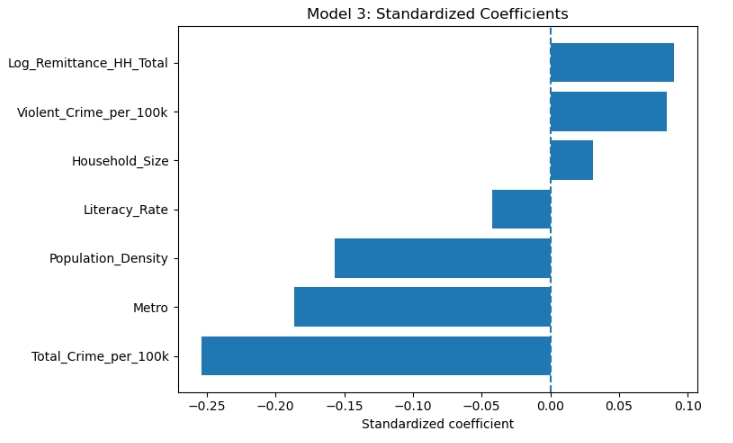
\includegraphics[width=0.85\textwidth]{Model_3_Standardized_Coefficients.jpeg}
\caption{Standardized Coefficients for Model 3}
\label{fig:appendix_standardized_coefficients}
\end{figure}



% ============================================================
% C Diagnostics
% ============================================================

\section{Diagnostics}

This appendix reports diagnostic checks for the main Model 3 specification.

\begin{table}[H]
\centering
\caption{Variance Inflation Factors for Model 3 Predictors}
\label{tab:appendix_vif}
\footnotesize
\begin{tabular}{lr}
\toprule
Variable & VIF \\
\midrule
Population Density & 2.5134 \\
Household Size & 1.6476 \\
Literacy Rate & 1.5239 \\
Total Crime per 100k & 2.6011 \\
Violent Crime per 100k & 1.7544 \\
Metro & 2.3910 \\
Log Remittance HH Total & 1.8707 \\
\bottomrule
\end{tabular}
\begin{flushleft}
\footnotesize Notes: The constant term is excluded from interpretation. All predictor VIF values are below 3, suggesting no serious multicollinearity problem.
\end{flushleft}
\end{table}


\begin{table}[H]
\centering
\caption{Model 3 Diagnostic Test Results}
\label{tab:appendix_diagnostics}
\footnotesize
\begin{tabular}{lrr}
\toprule
Test & Statistic & $p$-value \\
\midrule
Breusch-Pagan LM & 13.5821 & 0.0591 \\
Breusch-Pagan F & 1.9785 & 0.0579 \\
Jarque-Bera & 39.5323 & 0.0000 \\
Ramsey RESET & 0.3357 & 0.5628 \\
\bottomrule
\end{tabular}
\begin{flushleft}
\footnotesize Notes: The Breusch-Pagan result shows borderline evidence of heteroskedasticity, supporting the use of HC3 robust standard errors. The Jarque-Bera test indicates non-normal residuals. The Ramsey RESET result does not suggest major functional-form misspecification.
\end{flushleft}
\end{table}


\begin{table}[H]
\centering
\caption{Influential Observations in Model 3 Based on Cook's Distance}
\label{tab:appendix_cooks_observations}
\scriptsize
\begin{tabular}{lrrrr}
\toprule
Constituency & Margin Percentage & Fitted Value & Residual & Cook's Distance \\
\midrule
Rangamati-1 & 73.1731 & 20.6606 & 52.5124 & 0.0751 \\
Bandarban-1 & 68.7836 & 21.9964 & 46.7872 & 0.0605 \\
Chittagong-8 & 48.1303 & 21.8901 & 26.2402 & 0.0379 \\
Rangpur-3 & 35.0412 & 15.0835 & 19.9577 & 0.0249 \\
Dhaka-9 & 35.0709 & 10.2321 & 24.8389 & 0.0245 \\
Mymensingh-4 & 2.3919 & 22.5191 & -20.1273 & 0.0238 \\
Bogura-1 & 49.4688 & 15.7106 & 33.7582 & 0.0230 \\
Chittagong-6 & 61.2812 & 24.1318 & 37.1495 & 0.0225 \\
Bhola-3 & 43.5913 & 19.8319 & 23.7594 & 0.0215 \\
Patuakhali-1 & 44.6739 & 16.9377 & 27.7362 & 0.0211 \\
Chittagong-12 & 64.6446 & 24.5987 & 40.0459 & 0.0195 \\
Netrokona-4 & 60.2873 & 24.5905 & 35.6967 & 0.0190 \\
Bhola-4 & 39.8518 & 19.2074 & 20.6444 & 0.0153 \\
Chittagong-5 & 51.8816 & 24.0271 & 27.8545 & 0.0143 \\
Gaibandha-1 & 57.4795 & 18.3137 & 39.1658 & 0.0143 \\
Sylhet-2 & 51.4139 & 28.7403 & 22.6736 & 0.0130 \\
Pabna-2 & 47.8898 & 15.0172 & 32.8726 & 0.0118 \\
Lalmonirhat-3 & 42.5792 & 16.4647 & 26.1145 & 0.0115 \\
Tangail-2 & 53.0106 & 25.3374 & 27.6732 & 0.0114 \\
Jamalpur-4 & 53.2661 & 24.1940 & 29.0721 & 0.0111 \\
\bottomrule
\end{tabular}
\begin{flushleft}
\footnotesize Notes: Cook's distance identifies observations with relatively high influence on the fitted Model 3 results. The threshold used in the analysis was approximately 0.0135.
\end{flushleft}
\end{table}


\begin{figure}[H]
\centering
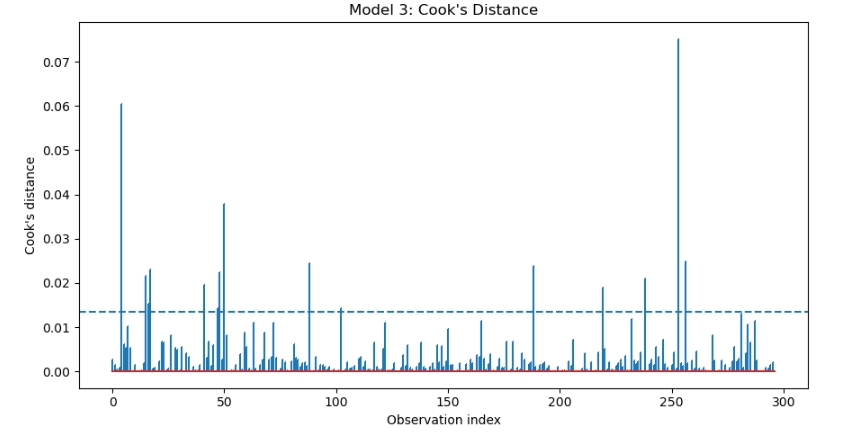
\includegraphics[width=0.90\textwidth]{Model_3_Diagnostic_Cooks_Distance.jpeg}
\caption{Cook's Distance Plot for Model 3}
\label{fig:appendix_cooks_distance}
\end{figure}


\begin{figure}[H]
\centering
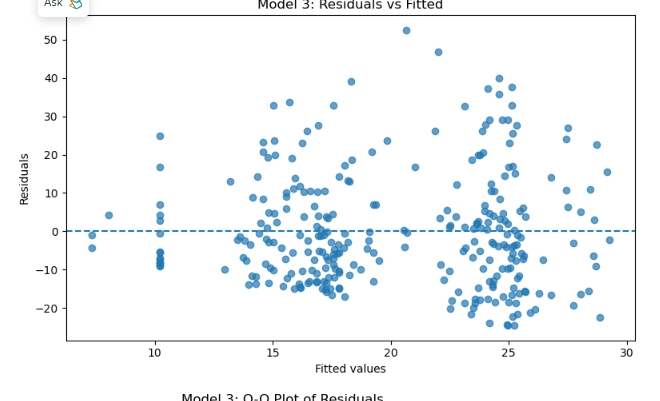
\includegraphics[width=0.90\textwidth]{Model_3_Diagnostic_Residuals_vs_Fitted.jpeg}
\caption{Residuals versus Fitted Values for Model 3}
\label{fig:appendix_residuals_fitted}
\end{figure}


\begin{figure}[H]
\centering
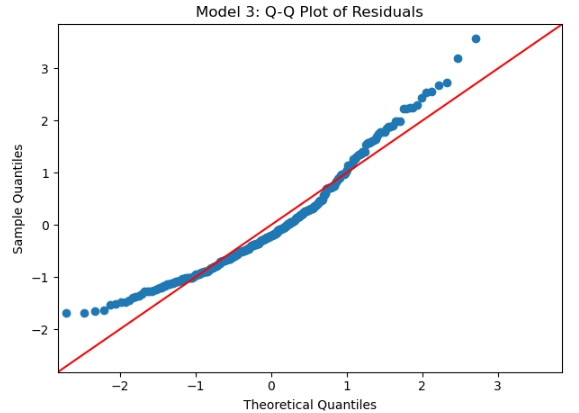
\includegraphics[width=0.90\textwidth]{Model_3_Diagnostic_QQ_Plot.jpeg}
\caption{Q-Q Plot of Model 3 Residuals}
\label{fig:appendix_qq_plot}
\end{figure}

\end{document}